\chapter{Architecture Constraints}
This chapter lists the constraints of the architecture. For instance, due to those constraints, some alternatives may not be evaluated and some decisions have to be made in a certain direction.
In particular, we will first describe the development environment. Second, we will identify the layers of the software architecture and locate SUM\_SOH in one specific layer. Finally, we will
present the generic component interface and we will conclude by evaluating other possible constraints and assumptions. 

\section{Environment}
\label{sec:environment}
\begin{longtable}{|l|l|l|}
\hline
\begin{minipage}{0.18\linewidth}\raggedright\vspace{.75ex}\textbf{Tool Name}\vspace{.75ex}\end{minipage} & \begin{minipage}{0.18\linewidth}\raggedright\vspace{.75ex}\textbf{Version}\vspace{.75ex}\end{minipage} & \begin{minipage}{0.55\linewidth}\raggedright\vspace{.75ex}\textbf{Description}\vspace{.75ex}\end{minipage}\\
\hline\hline
\endfirsthead
\hline
\begin{minipage}{0.18\linewidth}\raggedright\vspace{.75ex}\textbf{Tool Name}\vspace{.75ex}\end{minipage} & \begin{minipage}{0.18\linewidth}\raggedright\vspace{.75ex}\textbf{Version}\vspace{.75ex}\end{minipage} & \begin{minipage}{0.55\linewidth}\raggedright\vspace{.75ex}\textbf{Description}\vspace{.75ex}\end{minipage}\\
\hline\hline
\endhead
\hline
\endfoot
\hline
\endlastfoot
\begin{minipage}{0.18\linewidth}\raggedright\vspace{.75ex}ISOLAR-AB\vspace{.75ex}\end{minipage} & \begin{minipage}{0.18\linewidth}\raggedright\vspace{.75ex}12.3.3BETA1\vspace{.75ex}\end{minipage} & \begin{minipage}{0.55\linewidth}\raggedright\vspace{.75ex}AUTOSAR Authoring and BSW Configuration tools.\vspace{.75ex}\end{minipage}\\\hline
\begin{minipage}{0.18\linewidth}\raggedright\vspace{.75ex}RTA-BSW\vspace{.75ex}\end{minipage} & \begin{minipage}{0.18\linewidth}\raggedright\vspace{.75ex}12.3.3pr1\vspace{.75ex}\end{minipage} & \begin{minipage}{0.55\linewidth}\raggedright\vspace{.75ex}BSW automatic configuration and code generation.\vspace{.75ex}\end{minipage}\\\hline
\begin{minipage}{0.18\linewidth}\raggedright\vspace{.75ex}RTA-RTE\vspace{.75ex}\end{minipage} & \begin{minipage}{0.18\linewidth}\raggedright\vspace{.75ex}12.4.0\vspace{.75ex}\end{minipage} & \begin{minipage}{0.55\linewidth}\raggedright\vspace{.75ex}RTE generator used for testing\vspace{.75ex}\end{minipage}\\\hline
\begin{minipage}{0.18\linewidth}\raggedright\vspace{.75ex}RTA-OS\vspace{.75ex}\end{minipage} & \begin{minipage}{0.18\linewidth}\raggedright\vspace{.75ex}6.1.0\vspace{.75ex}\end{minipage} & \begin{minipage}{0.55\linewidth}\raggedright\vspace{.75ex} OS that is used for testing, as AUTOSAR OS\vspace{.75ex}\end{minipage}\\\hline
\begin{minipage}{0.18\linewidth}\raggedright\vspace{.75ex}MemMapGen\vspace{.75ex}\end{minipage} & \begin{minipage}{0.18\linewidth}\raggedright\vspace{.75ex}12.3.0\vspace{.75ex}\end{minipage} & \begin{minipage}{0.55\linewidth}\raggedright\vspace{.75ex} MemMap header file generator.\vspace{.75ex}\end{minipage}\\\hline
\begin{minipage}{0.18\linewidth}\raggedright\vspace{.75ex}Cantata\vspace{.75ex}\end{minipage} & \begin{minipage}{0.18\linewidth}\raggedright\vspace{.75ex}9.5\vspace{.75ex}\end{minipage} & \begin{minipage}{0.55\linewidth}\raggedright\vspace{.75ex}Used for functional testing\vspace{.75ex}\end{minipage}\\\hline
\end{longtable}

\section{Layers Definition}
The SUM\_SOH is a software module in the application layer of the standardized architecture of AUTOSAR (Figure~\ref{fig:Layers}). 
It interacts with other RTA-SUM modules and components of the BSW. In the latter case, the RTE is the means through which the interaction takes place.
\begin{figure}[htp]
\centering
	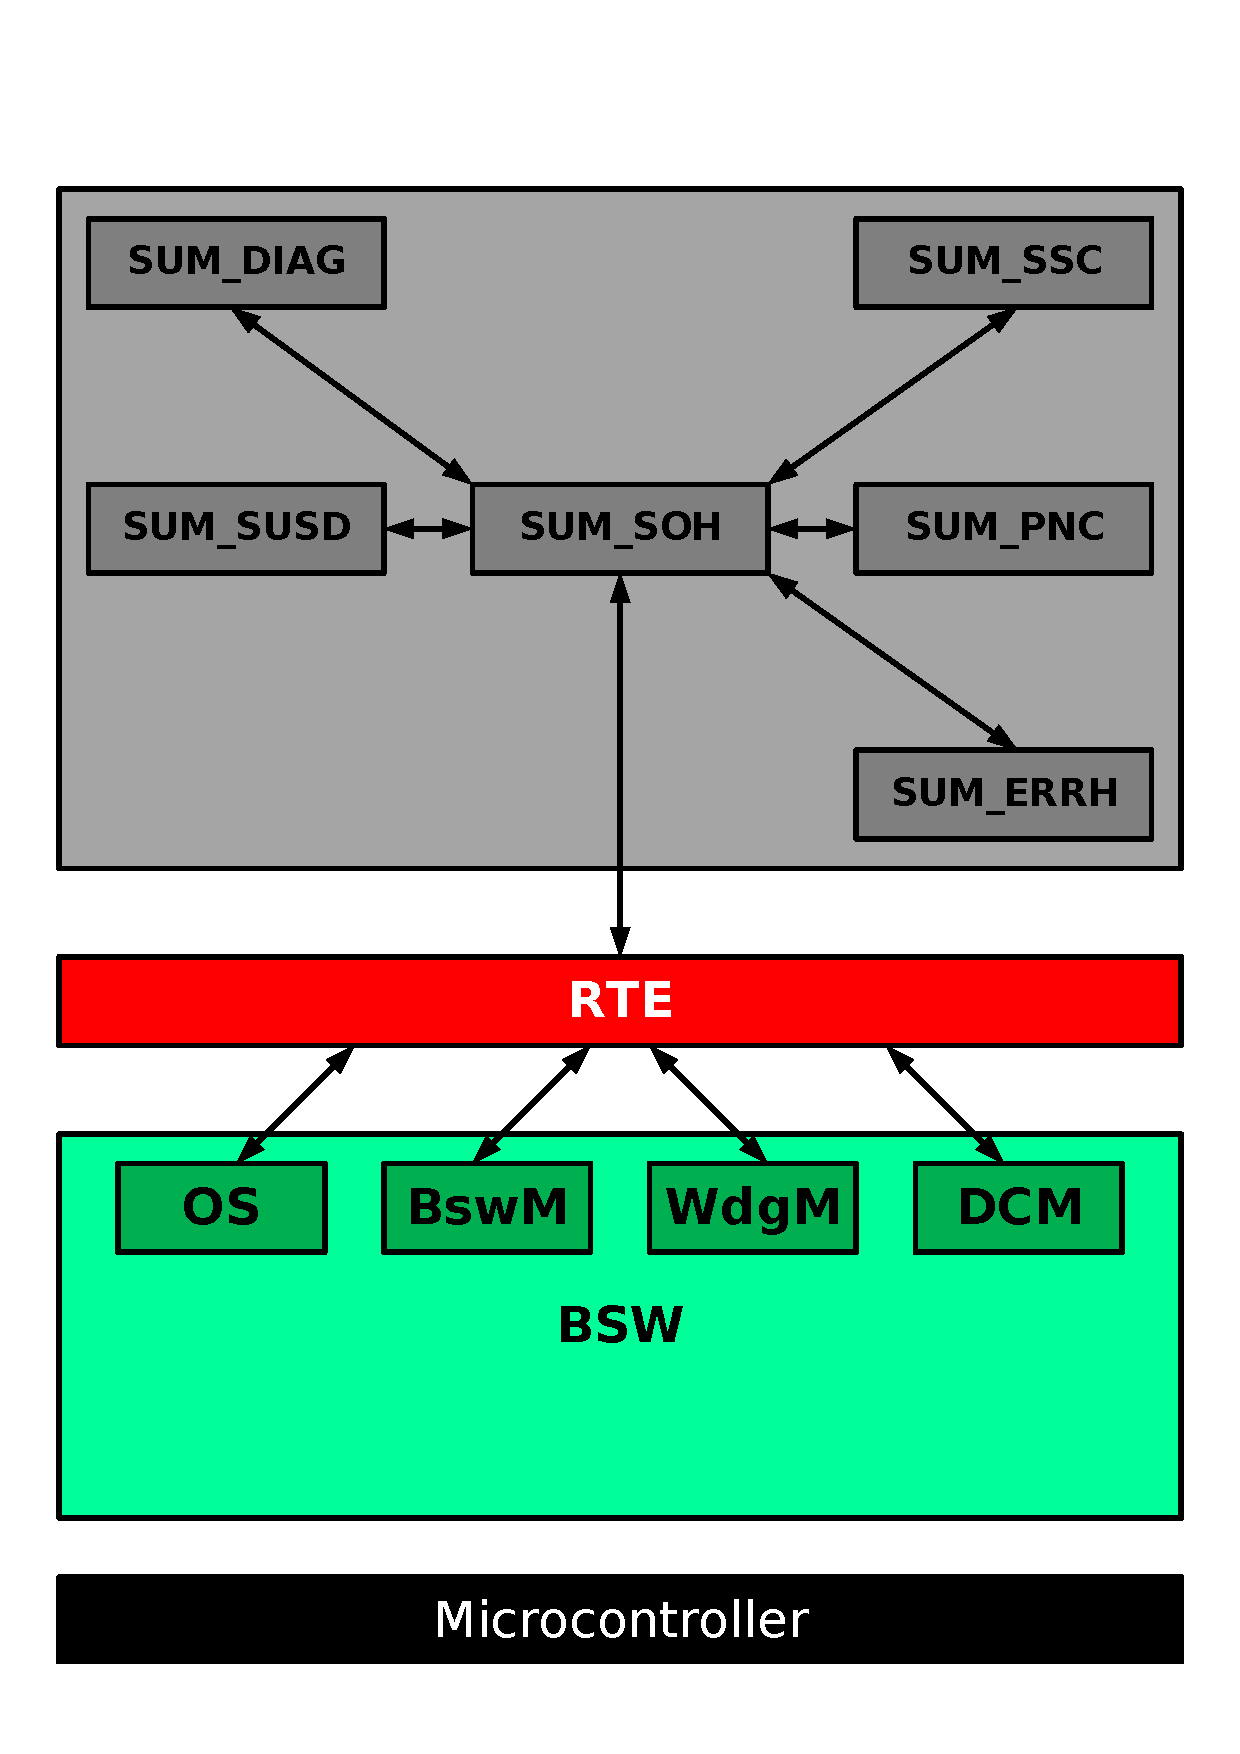
\includegraphics[scale=0.3]{images/Layers}
	\caption{System layer overview.}
	\label{fig:Layers}
\end{figure}

\section{Generic component interface}

Standard Utility Modules are dependent on each other for some functions. The SUM_SOH dependencies require that ECUs deploying the SUM_SOH shall also deploy the following SUMs: SUM\_DIAG, SUM\_SUSD, SUM\_SSC, SUM\_PNC and SUM\_ERRH. By means of the RTE, it also interacts with the OS, BswM, DCM and WdgM (Figure~\ref{fig:component}). .

\begin{figure}[htp]
\centering
	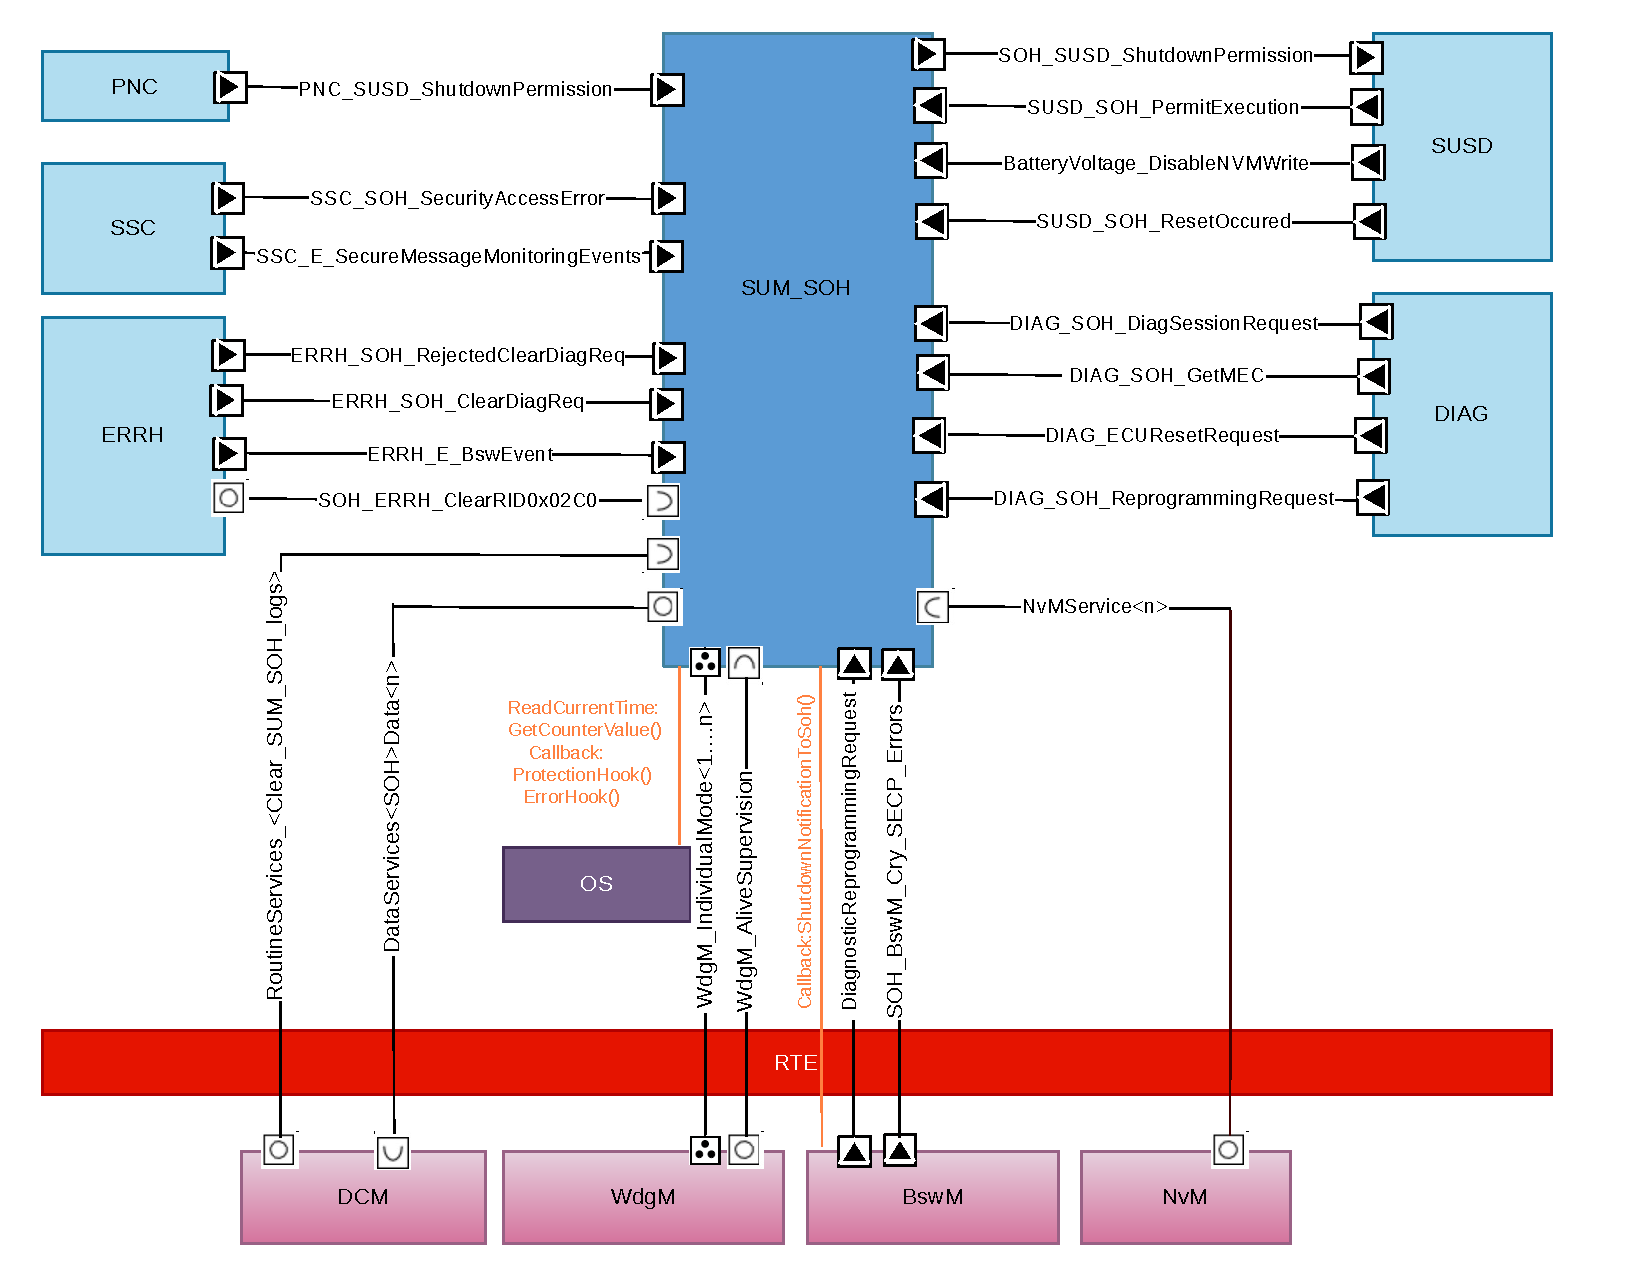
\includegraphics[width=\textwidth]{images/component}
	\caption{Generic Component Interface}
	\label{fig:component}
\end{figure}

Error detection based on host ECU type shall support BSW that fulfills the requirements of AUTOSAR_SWS_BasicSoftwareManager.
BSW that fulfills the requirements of AUTOSAR_SWS_COM.
BSW that fulfills the requirements of AUTOSAR_SWS_DiagnosticCommunicationManager.
BSW that fulfills the requirements of AUTOSAR_SWS_DiagnosticEventManager.
BSW that fulfills the requirements of AUTOSAR_SWS_WatchdogManager.
BSW that fulfills the requirements of AUTOSAR_SWS_NVRAMManager.
BSW that filfills the requirements of AUTOSAR_SWS_OS.


\subsection{Port Interfaces}
\label{sec:portinterfaces}
\Requirement{013}
{
All ECU types shall support Client / Server port interfaces.
All ECU types shall support Sender / Receiver port interfaces.
}
{
\Satisfies{SRS_SOH 016}
\Satisfies{SRS_SOH 228} 
\Satisfies{SRS_SOH 229}
\Satisfies{SRS_SOH 230} 
\Satisfies{SRS_SOH 232} 
\Satisfies{SRS_SOH 233}
\Satisfies{SRS_SOH 234} 
\Satisfies{SRS_SOH 235}
\Satisfies{SRS_SOH 248}
\Satisfies{SRS_SOH 249} 
\Satisfies{SRS_SOH 250} 
\Satisfies{SRS_SOH 253} 
\Satisfies{SRS_SOH 262}
}
\begin{longtable}{|l|l|l|l|l|}
\hline
\begin{minipage}{0.42\linewidth}\raggedright\vspace{.75ex}\textbf{Port Interface}\vspace{.75ex}\end{minipage} & \begin{minipage}{0.07\linewidth}\raggedright\vspace{.75ex}\textbf{Port Type}\vspace{.75ex}\end{minipage} & \begin{minipage}{0.10\linewidth}\raggedright\vspace{.75ex}\textbf{P-Port}\vspace{.75ex}\end{minipage} & \begin{minipage}{0.10\linewidth}\raggedright\vspace{.75ex}\textbf{R-Port}\vspace{.75ex}\end{minipage} & \begin{minipage}{0.17\linewidth}\raggedright\vspace{.75ex}\textbf{Description}\vspace{.75ex}\end{minipage}\\
\hline\hline
\endfirsthead
\hline
\begin{minipage}{0.42\linewidth}\raggedright\vspace{.75ex}\textbf{Port Interface}\vspace{.75ex}\end{minipage} & \begin{minipage}{0.07\linewidth}\raggedright\vspace{.75ex}\textbf{Port Type}\vspace{.75ex}\end{minipage} & \begin{minipage}{0.10\linewidth}\raggedright\vspace{.75ex}\textbf{P-Port}\vspace{.75ex}\end{minipage} & \begin{minipage}{0.10\linewidth}\raggedright\vspace{.75ex}\textbf{R-Port}\vspace{.75ex}\end{minipage} & \begin{minipage}{0.17\linewidth}\raggedright\vspace{.75ex}\textbf{Description}\vspace{.75ex}\end{minipage}\\
\hline\hline
\endhead
\hline
\endfoot
\hline
\endlastfoot
\begin{minipage}{0.42\linewidth}\raggedright\vspace{.75ex}ERRH\_E\_BswEvent\vspace{.75ex}\end{minipage} & \begin{minipage}{0.07\linewidth}\raggedright\vspace{.75ex}Sender / Receiver\vspace{.75ex}\end{minipage} & \begin{minipage}{0.10\linewidth}\raggedright\vspace{.75ex}SUM\_ERRH\vspace{.75ex}\end{minipage} & \begin{minipage}{0.10\linewidth}\raggedright\vspace{.75ex}SUM\_SOH\vspace{.75ex}\end{minipage} & \begin{minipage}{0.17\linewidth}\raggedright\vspace{.75ex}Reception of DEM events which are routed from SUM\_ERRH to the SUM\_SOH for processing.\vspace{.75ex}\end{minipage}\\\hline
\begin{minipage}{0.42\linewidth}\raggedright\vspace{.75ex}SUSD\_SOH\_PermitExecution\vspace{.75ex}\end{minipage} & \begin{minipage}{0.07\linewidth}\raggedright\vspace{.75ex}Sender / Receiver\vspace{.75ex}\end{minipage} & \begin{minipage}{0.10\linewidth}\raggedright\vspace{.75ex}SUM\_SUSD\vspace{.75ex}\end{minipage} & \begin{minipage}{0.10\linewidth}\raggedright\vspace{.75ex}SUM\_SOH\vspace{.75ex}\end{minipage} & \begin{minipage}{0.17\linewidth}\raggedright\vspace{.75ex}Permit Execution interface to indicate that operating conditions are correct for the SUM\_SOH to execute its functions.\vspace{.75ex}\end{minipage}\\\hline
\begin{minipage}{0.42\linewidth}\raggedright\vspace{.75ex}PNC\_SUSD\_ShutdownPermission\vspace{.75ex}\end{minipage} & \begin{minipage}{0.07\linewidth}\raggedright\vspace{.75ex}Sender / Receiver\vspace{.75ex}\end{minipage} & \begin{minipage}{0.10\linewidth}\raggedright\vspace{.75ex}SUM\_PNC\vspace{.75ex}\end{minipage} & \begin{minipage}{0.10\linewidth}\raggedright\vspace{.75ex}SUM\_SOH\vspace{.75ex}\end{minipage} & \begin{minipage}{0.17\linewidth}\raggedright\vspace{.75ex}Notification to the SUM\_SOH of any active or not active partial networks.\vspace{.75ex}\end{minipage}\\\hline
\begin{minipage}{0.42\linewidth}\raggedright\vspace{.75ex}SSC\_E\_SecureMessageMonitoringEvents\vspace{.75ex}\end{minipage} & \begin{minipage}{0.07\linewidth}\raggedright\vspace{.75ex}Sender / Receiver\vspace{.75ex}\end{minipage} & \begin{minipage}{0.10\linewidth}\raggedright\vspace{.75ex}SUM\_SSC\vspace{.75ex}\end{minipage} & \begin{minipage}{0.10\linewidth}\raggedright\vspace{.75ex}SUM\_SOH\vspace{.75ex}\end{minipage} & \begin{minipage}{0.17\linewidth}\raggedright\vspace{.75ex}Notification of MAC failures along with their types.\vspace{.75ex}\end{minipage}\\\hline
\begin{minipage}{0.42\linewidth}\raggedright\vspace{.75ex}DIAG\_ECUResetRequest\vspace{.75ex}\end{minipage} & \begin{minipage}{0.07\linewidth}\raggedright\vspace{.75ex}Sender / Receiver\vspace{.75ex}\end{minipage} & \begin{minipage}{0.10\linewidth}\raggedright\vspace{.75ex}SUM\_DIAG\vspace{.75ex}\end{minipage} & \begin{minipage}{0.10\linewidth}\raggedright\vspace{.75ex}SUM\_SOH\vspace{.75ex}\end{minipage} & \begin{minipage}{0.17\linewidth}\raggedright\vspace{.75ex}Notification of a service 0x11 tester-initiated request for ECU Reset (not programming).\vspace{.75ex}\end{minipage}\\\hline
\begin{minipage}{0.42\linewidth}\raggedright\vspace{.75ex}SUSD\_SOH\_ResetOccured\vspace{.75ex}\end{minipage} & \begin{minipage}{0.07\linewidth}\raggedright\vspace{.75ex}Sender / Receiver\vspace{.75ex}\end{minipage} & \begin{minipage}{0.10\linewidth}\raggedright\vspace{.75ex}SUM\_SUSD\vspace{.75ex}\end{minipage} & \begin{minipage}{0.10\linewidth}\raggedright\vspace{.75ex}SUM\_SOH\vspace{.75ex}\end{minipage} & \begin{minipage}{0.17\linewidth}\raggedright\vspace{.75ex}Notification to the SUM\_SOH that a reset occurred. The type of reset is also communicated to the SUM\_SOH. Type of resets may be delayed or immediate.\vspace{.75ex}\end{minipage}\\\hline
\begin{minipage}{0.42\linewidth}\raggedright\vspace{.75ex}SSFM\_ClearDiagReq\vspace{.75ex}\end{minipage} & \begin{minipage}{0.07\linewidth}\raggedright\vspace{.75ex}Sender / Receiver\vspace{.75ex}\end{minipage} & \begin{minipage}{0.10\linewidth}\raggedright\vspace{.75ex}SUM\_SSFM\vspace{.75ex}\end{minipage} & \begin{minipage}{0.10\linewidth}\raggedright\vspace{.75ex}SUM\_SOH\vspace{.75ex}\end{minipage} & \begin{minipage}{0.17\linewidth}\raggedright\vspace{.75ex}Notification to the SUM\_SOH that a service 0x04 or a service 0x14 request was accepted or rejected.\vspace{.75ex}\end{minipage}\\\hline
\begin{minipage}{0.42\linewidth}\raggedright\vspace{.75ex}DIAG\_SOH\_DiagSessionRequest\vspace{.75ex}\end{minipage} & \begin{minipage}{0.07\linewidth}\raggedright\vspace{.75ex}Sender / Receiver\vspace{.75ex}\end{minipage} & \begin{minipage}{0.10\linewidth}\raggedright\vspace{.75ex}SUM\_DIAG\vspace{.75ex}\end{minipage} & \begin{minipage}{0.10\linewidth}\raggedright\vspace{.75ex}SUM\_SOH\vspace{.75ex}\end{minipage} & \begin{minipage}{0.17\linewidth}\raggedright\vspace{.75ex}Notification to the SUM\_SOH that a reprogramming request took place (service 0x10 subfunction 0x02).\vspace{.75ex}\end{minipage}\\\hline
\begin{minipage}{0.42\linewidth}\raggedright\vspace{.75ex}SSC\_SOH\_SecurityAccessError\vspace{.75ex}\end{minipage} & \begin{minipage}{0.07\linewidth}\raggedright\vspace{.75ex}Sender / Receiver\vspace{.75ex}\end{minipage} & \begin{minipage}{0.10\linewidth}\raggedright\vspace{.75ex}SUM\_SSC\vspace{.75ex}\end{minipage} & \begin{minipage}{0.10\linewidth}\raggedright\vspace{.75ex}SUM\_SOH\vspace{.75ex}\end{minipage} & \begin{minipage}{0.17\linewidth}\raggedright\vspace{.75ex}Notification to the SUM\_SOH of the occurrences of service 0x27 failures.\vspace{.75ex}\end{minipage}\\\hline
\begin{minipage}{0.42\linewidth}\raggedright\vspace{.75ex}BatteryVoltage\_DisableNVMWrite\vspace{.75ex}\end{minipage} & \begin{minipage}{0.07\linewidth}\raggedright\vspace{.75ex}Sender / Receiver\vspace{.75ex}\end{minipage} & \begin{minipage}{0.10\linewidth}\raggedright\vspace{.75ex}SUM\_SUSD\vspace{.75ex}\end{minipage} & \begin{minipage}{0.10\linewidth}\raggedright\vspace{.75ex}SUM\_SOH\vspace{.75ex}\end{minipage} & \begin{minipage}{0.17\linewidth}\raggedright\vspace{.75ex}Notification to the SUM\_SOH from SUM\_SUSD that vehicle battery voltage is too low to perform NVM writes.\vspace{.75ex}\end{minipage}\\\hline
\begin{minipage}{0.42\linewidth}\raggedright\vspace{.75ex}DIAG\_GetMEC\vspace{.75ex}\end{minipage} & \begin{minipage}{0.07\linewidth}\raggedright\vspace{.75ex}Sender / Receiver\vspace{.75ex}\end{minipage} & \begin{minipage}{0.10\linewidth}\raggedright\vspace{.75ex}SUM\_DIAG\vspace{.75ex}\end{minipage} & \begin{minipage}{0.10\linewidth}\raggedright\vspace{.75ex}SUM\_SOH\vspace{.75ex}\end{minipage} & \begin{minipage}{0.17\linewidth}\raggedright\vspace{.75ex}This interface is used by the SUM\_DIAG to communicate to SUM\_SOH to value of the MEC.\vspace{.75ex}\end{minipage}\\\hline
\begin{minipage}{0.42\linewidth}\raggedright\vspace{.75ex}DataServices<SOH>Data<n>\vspace{.75ex}\end{minipage} & \begin{minipage}{0.07\linewidth}\raggedright\vspace{.75ex}Client / Server\vspace{.75ex}\end{minipage} & \begin{minipage}{0.10\linewidth}\raggedright\vspace{.75ex}DCM\vspace{.75ex}\end{minipage} & \begin{minipage}{0.10\linewidth}\raggedright\vspace{.75ex}SUM\_SOH\vspace{.75ex}\end{minipage} & \begin{minipage}{0.17\linewidth}\raggedright\vspace{.75ex}To support the collection of Diagnostic DIDs that are part of the SUM\_SOH functionalities.\vspace{.75ex}\end{minipage}\\\hline
\begin{minipage}{0.42\linewidth}\raggedright\vspace{.75ex}DiagnosticReprogrammingRequest\vspace{.75ex}\end{minipage} & \begin{minipage}{0.07\linewidth}\raggedright\vspace{.75ex}Mode Switch\vspace{.75ex}\end{minipage} & \begin{minipage}{0.10\linewidth}\raggedright\vspace{.75ex}BswM\vspace{.75ex}\end{minipage} & \begin{minipage}{0.10\linewidth}\raggedright\vspace{.75ex}SUM\_SOH\vspace{.75ex}\end{minipage} & \begin{minipage}{0.17\linewidth}\raggedright\vspace{.75ex}Notification of a request to shutdown to reset as part of programming to jump to boot.\vspace{.75ex}\end{minipage}\\\hline
\begin{minipage}{0.42\linewidth}\raggedright\vspace{.75ex}SOH\_WdgM\_IndividualMode<1...n>\vspace{.75ex}\end{minipage} & \begin{minipage}{0.07\linewidth}\raggedright\vspace{.75ex}Mode Switch\vspace{.75ex}\end{minipage} & \begin{minipage}{0.10\linewidth}\raggedright\vspace{.75ex}WdgM\vspace{.75ex}\end{minipage} & \begin{minipage}{0.10\linewidth}\raggedright\vspace{.75ex}SUM\_SOH\vspace{.75ex}\end{minipage} & \begin{minipage}{0.17\linewidth}\raggedright\vspace{.75ex}Notification of WdgM local supervision failures occurrence for all supervised entities excluding the SUM\_SOH and the SUM\_ERRH.\newline \footnotesize{These interfaces replace the SOH\_BswM\_WdgM \_IndividualMode<1...n> interfaces described in GB8002.}\vspace{.75ex}\end{minipage}\\\hline
\begin{minipage}{0.42\linewidth}\raggedright\vspace{.75ex}SOH\_WdgM\_IndividualMode\_Errh\vspace{.75ex}\end{minipage} & \begin{minipage}{0.07\linewidth}\raggedright\vspace{.75ex}Mode Switch\vspace{.75ex}\end{minipage} & \begin{minipage}{0.10\linewidth}\raggedright\vspace{.75ex}WdgM\vspace{.75ex}\end{minipage} & \begin{minipage}{0.10\linewidth}\raggedright\vspace{.75ex}SUM\_SOH\vspace{.75ex}\end{minipage} & \begin{minipage}{0.17\linewidth}\raggedright\vspace{.75ex}Notification of the WdgM SUM\_ERRH local supervision failures occurrences. \newline \footnotesize{This interface replaces the SOH\_BsWM\_WdgM \_ERRHMode interface described in GB8002.}\vspace{.75ex}\end{minipage}\\\hline
\begin{minipage}{0.42\linewidth}\raggedright\vspace{.75ex}RP\_ErrorStatus\vspace{.75ex}\end{minipage} & \begin{minipage}{0.07\linewidth}\raggedright\vspace{.75ex}Mode Switch\vspace{.75ex}\end{minipage} & \begin{minipage}{0.10\linewidth}\raggedright\vspace{.75ex}BswM\vspace{.75ex}\end{minipage} & \begin{minipage}{0.10\linewidth}\raggedright\vspace{.75ex}SOH\vspace{.75ex}\end{minipage} & \begin{minipage}{0.17\linewidth}\raggedright\vspace{.75ex}This interface is used by the BswM to notify SUM\_SOH of SecP errors occurrences.\vspace{.75ex}\end{minipage}\\\hline
\begin{minipage}{0.42\linewidth}\raggedright\vspace{.75ex}NvMService\vspace{.75ex}\end{minipage} & \begin{minipage}{0.07\linewidth}\raggedright\vspace{.75ex}Client / Server\vspace{.75ex}\end{minipage} & \begin{minipage}{0.10\linewidth}\raggedright\vspace{.75ex}NvM\vspace{.75ex}\end{minipage} & \begin{minipage}{0.10\linewidth}\raggedright\vspace{.75ex}SOH\vspace{.75ex}\end{minipage} & \begin{minipage}{0.17\linewidth}\raggedright\vspace{.75ex}The interface provides services for the management and maintenance of NV data related to SOH Metrics.\vspace{.75ex}\end{minipage}\\\hline
\begin{minipage}{0.42\linewidth}\raggedright\vspace{.75ex}TCS\_SWC\_Clock\vspace{.75ex}\end{minipage} & \begin{minipage}{0.07\linewidth}\raggedright\vspace{.75ex}Client / Server\vspace{.75ex}\end{minipage} & \begin{minipage}{0.10\linewidth}\raggedright\vspace{.75ex}TCS\vspace{.75ex}\end{minipage} & \begin{minipage}{0.10\linewidth}\raggedright\vspace{.75ex}SOH\vspace{.75ex}\end{minipage} & \begin{minipage}{0.17\linewidth}\raggedright\vspace{.75ex}Provides Global Time for timestamp (unit 100ms).\vspace{.75ex}\end{minipage}\\\hline
\begin{minipage}{0.42\linewidth}\raggedright\vspace{.75ex}RoutineServices\_Clear\_SUM\_SOH\_logs\vspace{.75ex}\end{minipage} & \begin{minipage}{0.07\linewidth}\raggedright\vspace{.75ex}Client / Server\vspace{.75ex}\end{minipage} & \begin{minipage}{0.10\linewidth}\raggedright\vspace{.75ex}DCM\vspace{.75ex}\end{minipage} & \begin{minipage}{0.10\linewidth}\raggedright\vspace{.75ex}SOH\vspace{.75ex}\end{minipage} & \begin{minipage}{0.17\linewidth}\raggedright\vspace{.75ex}The interface provides services for the clear of the SOH Metrics.\vspace{.75ex}\end{minipage}\\\hline
\begin{minipage}{0.42\linewidth}\raggedright\vspace{.75ex}WdgM\_LocalSupervision\vspace{.75ex}\end{minipage} & \begin{minipage}{0.07\linewidth}\raggedright\vspace{.75ex} Client / Server\vspace{.75ex}\end{minipage} & \begin{minipage}{0.10\linewidth}\raggedright\vspace{.75ex}WdgM\vspace{.75ex}\end{minipage} & \begin{minipage}{0.10\linewidth}\raggedright\vspace{.75ex}SUM\_SOH\vspace{.75ex}\end{minipage} & \begin{minipage}{0.17\linewidth}\raggedright\vspace{.75ex}Notify the checkpoint reachement for implementing the Local Supervision.\vspace{.75ex}\end{minipage}\\\hline
\begin{minipage}{0.42\linewidth}\raggedright\vspace{.75ex}SOH\_ERRH\_ClearRID0x02C0\vspace{.75ex}\end{minipage} & \begin{minipage}{0.07\linewidth}\raggedright\vspace{.75ex}Client / Server\vspace{.75ex}\end{minipage} & \begin{minipage}{0.10\linewidth}\raggedright\vspace{.75ex}SUM\_ERRH\vspace{.75ex}\end{minipage} & \begin{minipage}{0.10\linewidth}\raggedright\vspace{.75ex}SUM\_SOH\vspace{.75ex}\end{minipage} & \begin{minipage}{0.17\linewidth}\raggedright\vspace{.75ex}The interface provides service for starting clear, all the metrics related to SUM\_SOH Local Supervision Detector implemented at ERRH side.\vspace{.75ex}\end{minipage}\\\hline
\begin{minipage}{0.42\linewidth}\raggedright\vspace{.75ex}SOH\_SUSD\_ShutdownPermission\vspace{.75ex}\end{minipage} & \begin{minipage}{0.07\linewidth}\raggedright\vspace{.75ex}Sender / Receiver\vspace{.75ex}\end{minipage} & \begin{minipage}{0.10\linewidth}\raggedright\vspace{.75ex}SUM\_SOH\vspace{.75ex}\end{minipage} & \begin{minipage}{0.10\linewidth}\raggedright\vspace{.75ex}SUM\_SUSD\vspace{.75ex}\end{minipage} & \begin{minipage}{0.17\linewidth}\raggedright\vspace{.75ex}Shutdown Permission interface to indicate that operating conditions are correct for the SUM\_SOH to execute the shutdown.\vspace{.75ex}\end{minipage}\\\hline
\end{longtable}



\section{Other constraints and assumptions}
\label{sec:otherconstraint}
The ECU in which the SUM_SOH is implemented shall have a Secure cumulative NVM memory type, as defined in CTRS section 7.1.6, accessible to the SUM_SOH.
The ECU in which the SUM_SOH is implemented shall have NonClearedRAM memory type accessible to the SUM_SOH.
The ECU in which the SUM_SOH is implemented shall have an AdaptableNVM memory type accessible to the SUM_SOH.

The ECU initialization sequence shall be implemented such that any NVM needed for the SUM_SOH function is available prior to the SUM_SOH being initialized.

For ECUs that implement Memory Partitioning mechanisms, the SUM_SOH shall be implemented in the supervisory partition of the ECU software. Rationale: SUM_SOH must be in the trusted partition in order to interface with OS services. Supervisory partition is expected to include BSW Modules.

The SUM_SOH shall be implemented as a Supervised Entity of the Watchdog Manager.

For the SUM_SOH DIDs, the relative Dcm parameter \textit{DcmDspDataUsePort} must be set to CLIENT\_SERVER. Starting from this configuration,
SUM_SOH will populate the DIDs values in a BIG\_ENDIAN format as it is expected at the UDS layer (because the \textit{DcmDspDataEndianness}  has no effect if CLIENT\_SERVER is selected for \textit{DcmDspDataUsePort}).